%% @Author: Ines Abdeljaoued Tej
%  @Date:   2018-06
%% @Class:  Graduation Project, ESSAI - Carthage University, Tunisia.


\section{Diagramme de cas d'utilisation}


\subsubsection{Premier pas vers la conception :}

\begin{enumerate}
    \item \textbf{Entités}:\\
    \begin{itemize}
        \item Administrateur : responsable de la gestion globale de "Safari".\\
        \item L'utilisateur : des bloggeurs avec un accès limité.\\
    \end{itemize}
    
    \item \textbf{Cas d'utilisation}:\\
    \renewcommand{\thefigure}{1}
    \renewcommand{\thetable}{1}
\begin{table}[htbp] % You can adjust the placement options as needed
    \centering
    
    \begin{tabular}{|l|l|}
        \hline
        \textbf{Entités} & \textbf{Cas D’utilisations}               \\ \hline
        Utilisateur   & Gèrer son profile                       \\
                         & S’athentifier                              \\
                         & Gèrer son poste \\ 
                         & Ajouter                                   \\
                         & Modifier                                  \\
                         & Supprimer                                 \\ \hline
        Administrateur    & S’athentifier                                                         \\
                         & Gèrer les users                 \\
                         & Ajouter un user                                   \\
                         & Modifier un user                                  \\
                         & Supprimer un user                                 \\ \hline
    \end{tabular}
    \caption{Tableau regroupant : Entités - Cas D'utilisation}
    \label{tab:entities_use_cases}
\end{table}

\paragraph{\\}
\setcounter{figure}{0} % Reset figure counter to 0
\begin{figure}[htbp]
    \centering
    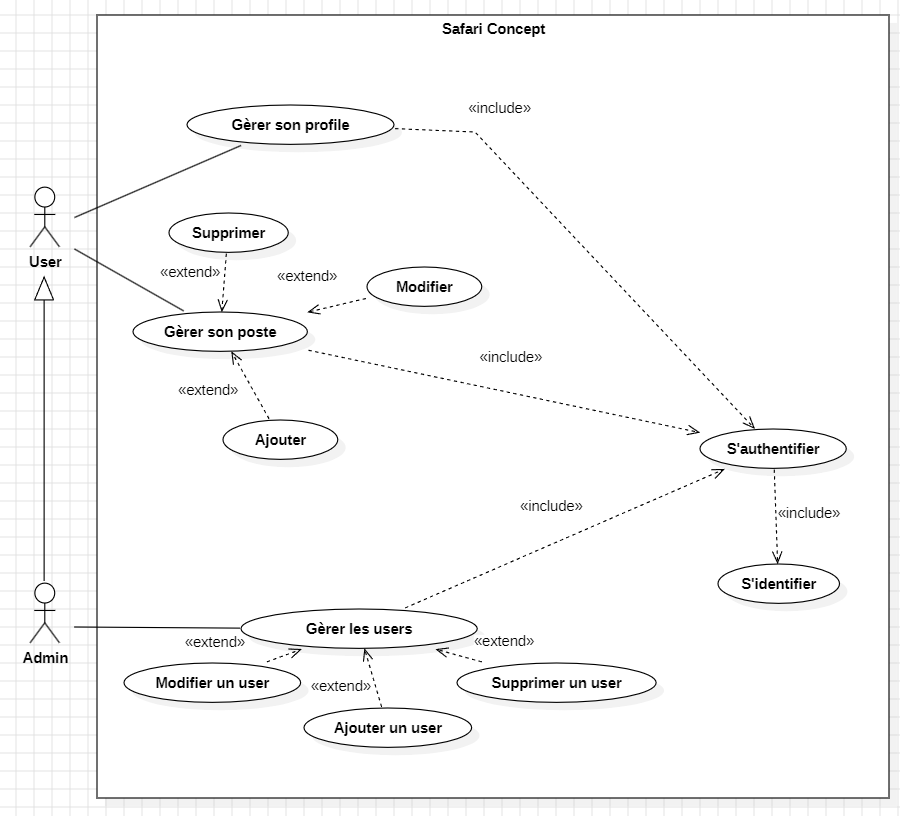
\includegraphics[width=0.9\textwidth]{images/image.png} 
    \caption{Diagramme de cas d'utilisation - "Safari"}
    \label{fig:Diagramme de cas d'utilisation - "Safari"}
\end{figure}

\paragraph{\\}

\section{Diagramme de Classe - "Safari"}

Le diagramme de classe est l’un des diagrammes les plus importants au 
niveau de la modélisation du logiciel/application, il montre non seulement 
la structure interne du système mais également une représentation 
abstraite des objets ( classes ) qui vont interagir entre eux.\\

Une classe est une description d’un groupe d’objet partageant un 
ensemble commun de propriétés, de comportements et de relations avec 
d’autres objets. Pour faire simple, il s’agit de :  Méthode ( autrement appelé opération ) - Attributs - Associations. \\

 \renewcommand{\thefigure}{2}
\begin{figure}[htbp]
    \centering
   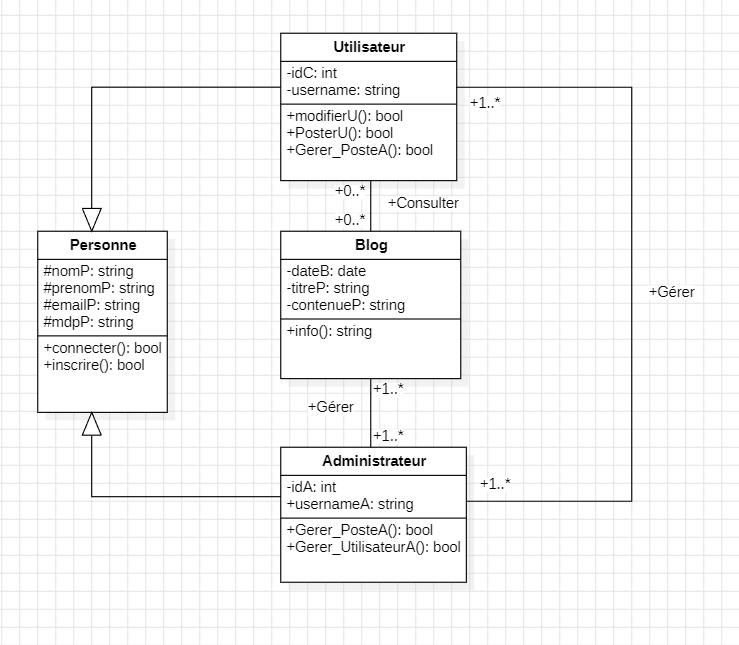
\includegraphics[width=0.8\textwidth]{images/image1.png} 
    \caption{Diagramme de Classe - "Safari"}

\subsubsection{Analyse et Lecture  :}

C’est pout cela, afin d’optimiser le diagramme on a décidé de mettre les 
points en commun dans une seule classe nommée Personne, ce dernier 
sera hérité par l'Utilisateur \& Administrateur. 
    \label{fig:Diagramme de classe - "Safari"}
\end{figure}

\end{enumerate}
